\clearpage
\chapter{Results and Analysis}
\section{Evaluation setup}
The main experiment compares the proposed cross-slice model ($K=5$) with the 2D U-Net baseline ($K=1$) using five-fold patient-level cross-validation over all 369 BraTS 2020 training patients. In each fold, both models are trained on the same 265 or 266 training patients, select their checkpoint on the same 30 validation patients, and are evaluated once on the same 73 or 74 test patients, so that every patient is a test patient exactly once and is segmented by both models. The two configurations share the training recipe of Chapter~5 (AdamW, learning rate $2 \times 10^{-4}$, Dice+BCE with $\lambda = 0.5$, five-fold tumour oversampling, base width 48, two transformer layers for $K=5$, batch 32, 30 epochs of 400 iterations, cosine schedule, EMA) and the same seed; the only difference is the number of input slices and, with it, the presence of the cross-slice transformer. All runs were executed on Astra A100 GPUs, with two or three runs sharing a GPU. In every run validation never triggered early stopping, so both models received exactly the same training budget of 30 epochs.

Several safeguards protect the validity of the comparison. Splitting is by patient, so slices of one patient never appear in two subsets. The test patients are used only once, after training; checkpoint selection and the ET post-processing threshold are chosen on validation patients. Metrics are computed per patient on whole volumes, which prevents slice-level averaging from hiding errors on healthy slices. Significance is assessed with paired tests on the same patients rather than by comparing means of independent samples. The training settings of the main experiment were fixed before it was run, taken from the mid-review design study, and confirmed as near-optimal by the Optuna search (Section~\ref{sec:optuna}).

\section{Evaluation criteria}
\textbf{Dice similarity coefficient.} For a region with predicted voxel set $P$ and ground-truth set $G$ in one patient's volume,
\begin{equation}
\mathrm{Dice} = \frac{2\,|P \cap G|}{|P| + |G|},
\end{equation}
which ranges from 0 (no overlap) to 1 (perfect overlap). Following the BraTS convention, if both $P$ and $G$ are empty the Dice is 1, and if exactly one is empty it is 0. Dice is computed separately for WT, TC and ET, and the mean Dice is their average. It is the primary metric.

\textbf{95th-percentile Hausdorff distance (HD95).} With $\partial P$ and $\partial G$ the surface voxels of the two regions, HD95 is the 95th percentile of the set of distances from each surface voxel of one region to the nearest surface voxel of the other, taken in both directions. It measures boundary error in millimetres (voxels are 1~mm isotropic); lower is better. If exactly one region is empty, the BraTS penalty of 373.13~mm is used, and if both are empty the distance is 0.

\textbf{False-positive slices.} The number of axial slices in a patient's volume on which tumour (WT) is predicted although the ground truth contains no tumour. It directly measures the slice-to-slice consistency that cross-slice context is meant to improve.

\textbf{Aggregation and statistics.} Each metric is computed per patient and averaged with equal weight per patient. We report the mean and standard deviation of the five fold-level averages, and the pooled per-patient mean over all 369 patients. Differences between $K=5$ and $K=1$ are tested with the two-sided Wilcoxon signed-rank test on the 369 paired per-patient values, which does not assume normally distributed differences. We also report the percentage of patients for which $K=5$ is strictly better.

\section{Result}
\subsection{Main five-fold comparison}
Table~\ref{tab:main} summarises the main result. Averaged over the five folds, the cross-slice model improves the Dice of all three regions and reduces the boundary error of all three regions as well as the number of false-positive slices. Figure~\ref{fig:folds} shows that the mean Dice of $K=5$ is higher than that of $K=1$ in four of the five folds, the exception being fold 1 (0.818 against 0.824). The WT Dice is higher in all five folds. The per-fold values are listed in Table~\ref{tab:perfold}.

\begin{table}[htbp]\centering\small
\caption{Five-fold cross-validation results on all 369 patients (mean $\pm$ standard deviation of the five fold averages; $\uparrow$ higher is better, $\downarrow$ lower is better)}\label{tab:main}
\resizebox{\textwidth}{!}{\begin{tabular}{lccc}\toprule
\textbf{Metric} & \textbf{Baseline 2D U-Net ($K=1$)} & \textbf{Cross-slice transformer ($K=5$)} & \textbf{Folds improved}\\\midrule
WT Dice $\uparrow$ & $0.898 \pm 0.010$ & $\mathbf{0.904 \pm 0.006}$ & 5 / 5\\
TC Dice $\uparrow$ & $0.837 \pm 0.021$ & $\mathbf{0.840 \pm 0.028}$ & 2 / 5\\
ET Dice $\uparrow$ & $0.783 \pm 0.042$ & $\mathbf{0.789 \pm 0.041}$ & 4 / 5\\
Mean Dice $\uparrow$ & $0.839 \pm 0.020$ & $\mathbf{0.844 \pm 0.022}$ & 4 / 5\\\midrule
HD95 WT (mm) $\downarrow$ & $7.7 \pm 1.0$ & $\mathbf{5.9 \pm 0.6}$ & 4 / 5\\
HD95 TC (mm) $\downarrow$ & $9.6 \pm 4.5$ & $\mathbf{7.9 \pm 4.9}$ & 4 / 5\\
HD95 ET (mm) $\downarrow$ & $33.4 \pm 19.0$ & $\mathbf{28.3 \pm 15.6}$ & 5 / 5\\
False-positive slices $\downarrow$ & $2.46 \pm 1.04$ & $\mathbf{1.62 \pm 0.43}$ & 3 / 5\\\midrule
Parameters & 4.33~M & 6.70~M & --\\
Training time per run (A100, shared) & 0.7--1.0 h & 1.3--2.0 h & --\\\bottomrule
\end{tabular}}
\end{table}

\begin{figure}[htbp]\centering
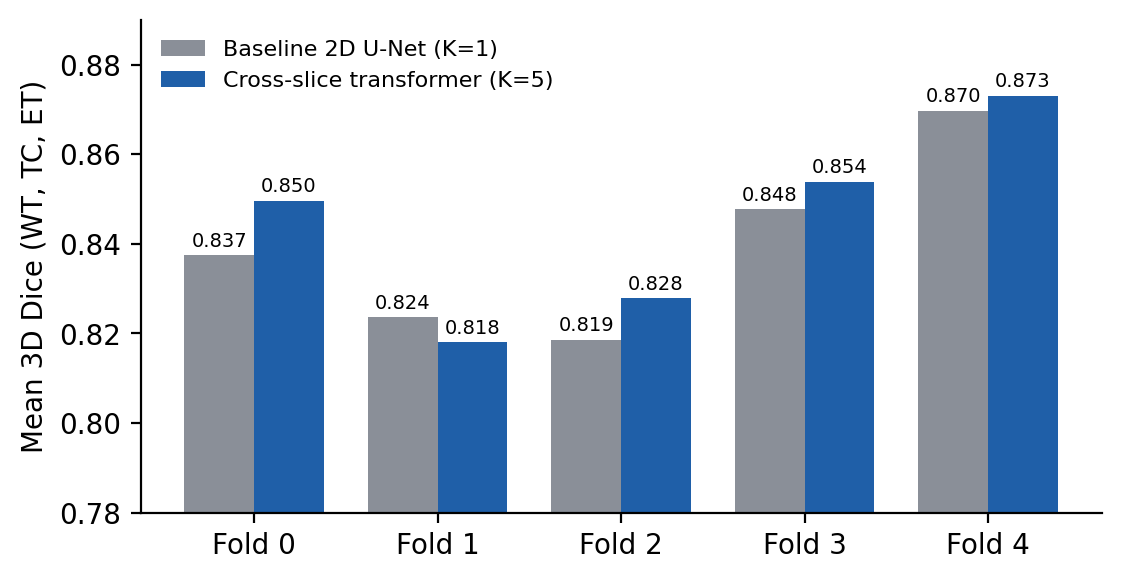
\includegraphics[width=0.85\textwidth]{figures/fold_mean_dice.png}
\caption{Mean 3D Dice per cross-validation fold for the baseline and the proposed model}\label{fig:folds}
\end{figure}

\begin{table}[htbp]\centering\small
\caption{Per-fold test results (73--74 patients per fold)}\label{tab:perfold}
\resizebox{\textwidth}{!}{\begin{tabular}{c|cccc|cccc}\toprule
 & \multicolumn{4}{c|}{\textbf{Baseline ($K=1$)}} & \multicolumn{4}{c}{\textbf{Proposed ($K=5$)}}\\
\textbf{Fold} & WT & TC & ET & HD95 WT & WT & TC & ET & HD95 WT\\\midrule
0 & 0.891 & 0.849 & 0.772 & 7.2 & 0.905 & 0.867 & 0.777 & 6.5\\
1 & 0.884 & 0.810 & 0.776 & 6.5 & 0.894 & 0.807 & 0.753 & 6.5\\
2 & 0.903 & 0.826 & 0.727 & 8.5 & 0.907 & 0.824 & 0.753 & 5.8\\
3 & 0.908 & 0.835 & 0.800 & 9.0 & 0.910 & 0.830 & 0.821 & 5.6\\
4 & 0.902 & 0.866 & 0.841 & 7.4 & 0.905 & 0.872 & 0.842 & 5.1\\\bottomrule
\end{tabular}}
\end{table}

\subsection{Paired per-patient analysis}
Table~\ref{tab:paired} pools all 369 patients and compares the two models patient by patient. All Dice differences favour the cross-slice model and are statistically significant ($p < 10^{-5}$), although they are small in magnitude: $+0.006$ for WT and ET and $+0.003$ for TC. The proposed model achieves a higher WT Dice for 71.5\% of patients and a higher mean Dice for 68.8\% of patients. The boundary metrics show larger relative gains: the mean HD95 decreases by 1.8~mm for WT (23\% lower), 1.6~mm for TC and 5.1~mm for ET (15\% lower), and the mean number of false-positive slices per patient decreases from 2.46 to 1.62 (34\% lower), all significant at the 5\% level. Figure~\ref{fig:paired} shows the distribution of the per-patient differences. For most patients the differences are close to zero, and the improvement in the means comes from a consistent small shift in Dice together with the removal of large boundary errors in a minority of difficult cases. This explains why the median HD95 changes little while the mean falls substantially.

\begin{table}[htbp]\centering\small
\caption{Paired per-patient comparison over all 369 patients (difference = $K=5$ minus $K=1$; two-sided Wilcoxon signed-rank test)}\label{tab:paired}
\resizebox{\textwidth}{!}{\begin{tabular}{lccccc}\toprule
\textbf{Metric} & \textbf{$K=1$ mean} & \textbf{$K=5$ mean} & \textbf{Mean difference} & \textbf{Patients improved} & \textbf{$p$-value}\\\midrule
WT Dice & 0.898 & 0.904 & $+0.006$ & 71.5\% & $7 \times 10^{-18}$\\
TC Dice & 0.837 & 0.840 & $+0.003$ & 63.1\% & $2 \times 10^{-6}$\\
ET Dice & 0.783 & 0.789 & $+0.006$ & 55.6\% & $3 \times 10^{-6}$\\
Mean Dice & 0.839 & 0.844 & $+0.005$ & 68.8\% & $8 \times 10^{-11}$\\
HD95 WT (mm) & 7.71 & 5.91 & $-1.80$ & 53.7\% & $2 \times 10^{-11}$\\
HD95 TC (mm) & 9.57 & 7.92 & $-1.65$ & 39.8\% & 0.032\\
HD95 ET (mm) & 33.46 & 28.39 & $-5.07$ & 24.7\% & 0.016\\
False-positive slices & 2.46 & 1.62 & $-0.83$ & 33.6\% & $2 \times 10^{-7}$\\\bottomrule
\end{tabular}}

\vspace{2pt}\footnotesize ``Patients improved'' counts strict improvements; for HD95 and false-positive slices many patients tie (for example, zero false-positive slices for both models).
\end{table}

\begin{figure}[htbp]\centering
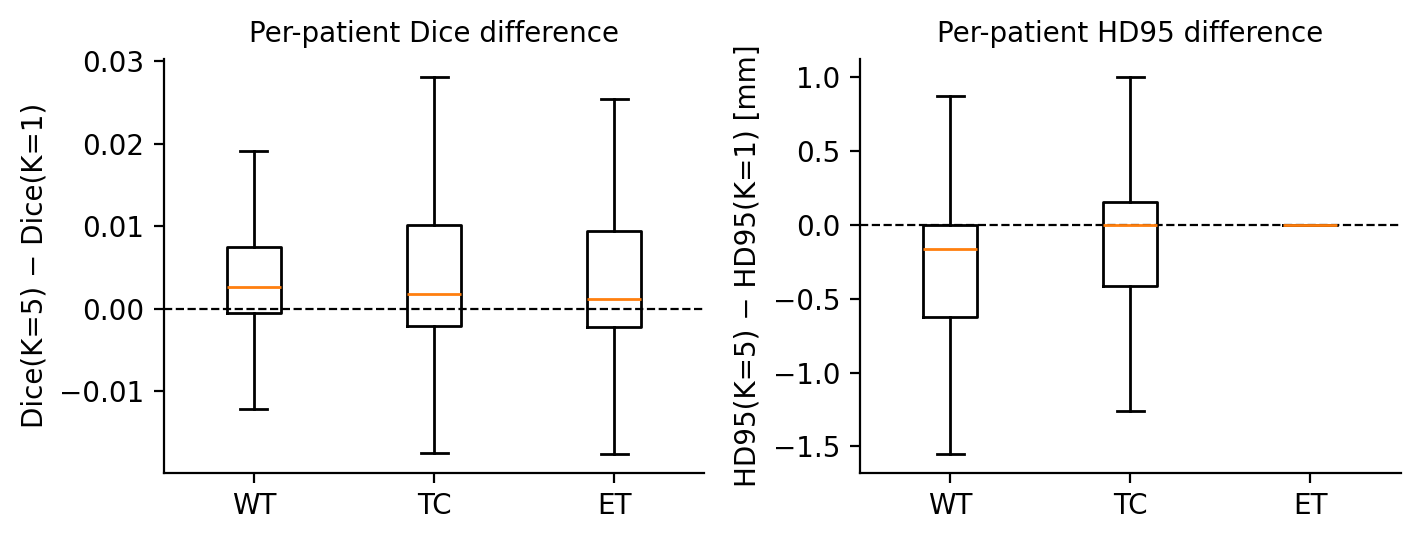
\includegraphics[width=\textwidth]{figures/paired_diff.png}
\caption{Distribution of per-patient differences between the proposed model and the baseline over 369 patients (boxes show the interquartile range; outliers omitted)}\label{fig:paired}
\end{figure}

\begin{figure}[htbp]\centering
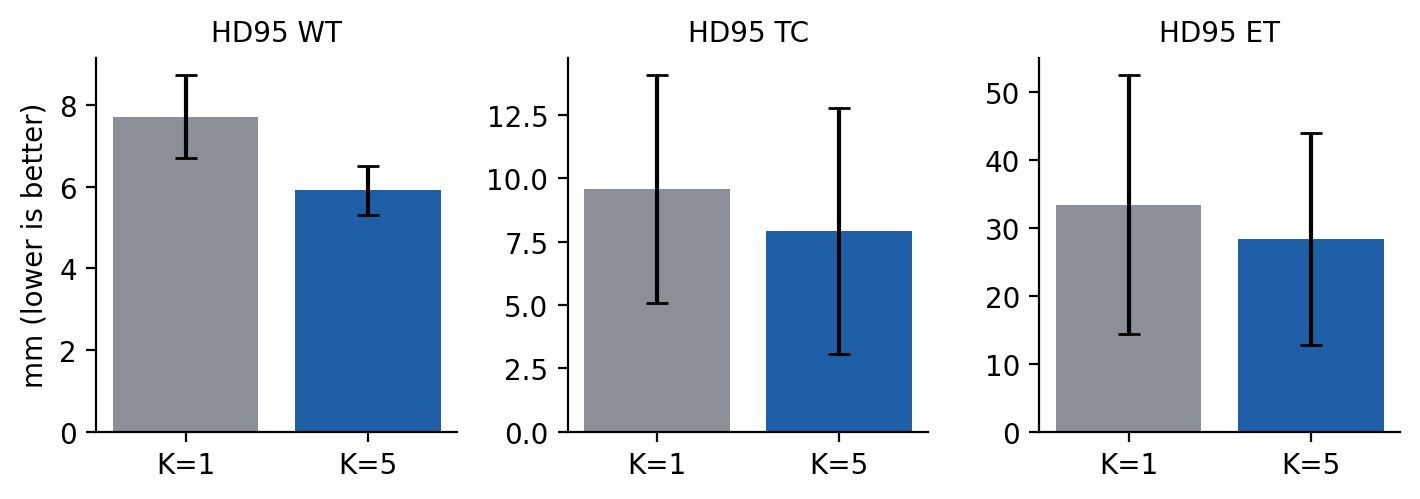
\includegraphics[width=0.95\textwidth]{figures/hd95.png}
\caption{HD95 boundary error per region (mean and standard deviation over the five folds)}\label{fig:hd95}
\end{figure}

\subsection{Training behaviour}
Figure~\ref{fig:curves} shows the training loss and the validation mean 3D Dice for fold 0. Both models converge smoothly. The baseline reached its best validation score at epoch 16, while the cross-slice model continued to improve until epoch 28, as the learning rate approached zero. In folds 1--4 the best validation epoch of the cross-slice model was between 14 and 18 and that of the baseline between 14 and 16. Training a $K=5$ model took 1.3--2.0 hours and a $K=1$ model 0.7--1.0 hours on a shared A100, with peak GPU memory of 12.5~GB and 3.8~GB respectively. The ET size threshold selected on validation patients ranged from 0 to 1,000 voxels across runs.

\begin{figure}[htbp]\centering
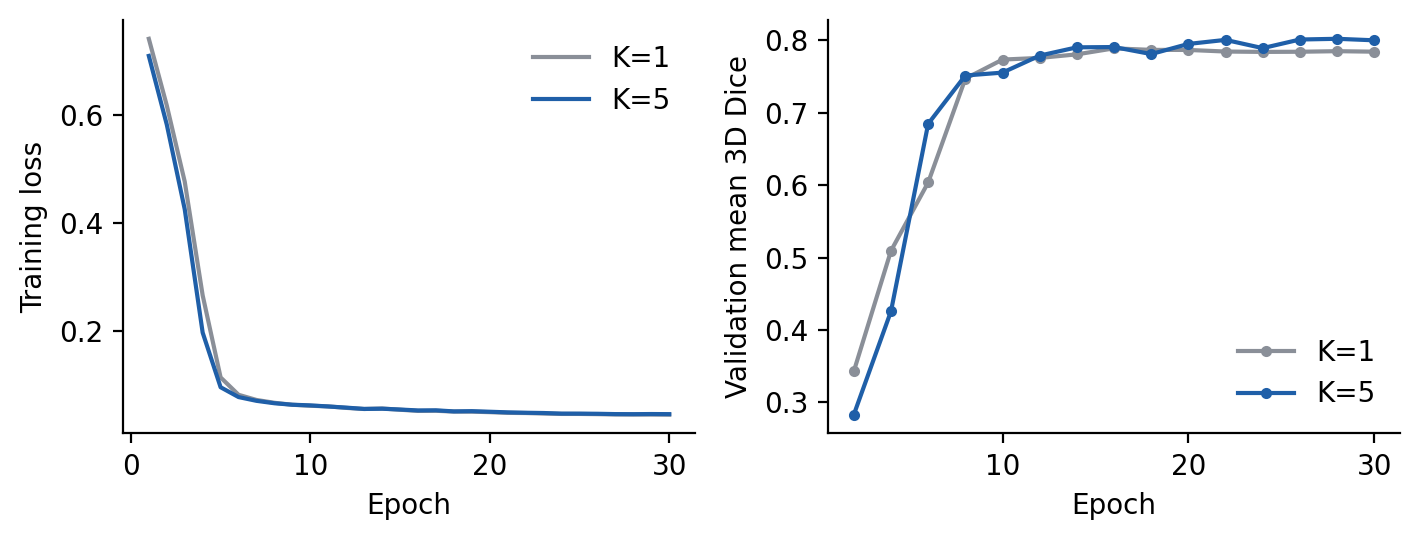
\includegraphics[width=\textwidth]{figures/training_curves.png}
\caption{Training loss and validation mean 3D Dice per epoch on fold 0}\label{fig:curves}
\end{figure}

\subsection{Automated hyper-parameter search}\label{sec:optuna}
The Optuna search ran ten trials in its one-hour budget: six completed and four were pruned early. Figure~\ref{fig:optuna} and Table~\ref{tab:optuna} summarise them. The best trial used $K=5$, a learning rate of $1.76 \times 10^{-4}$, weight decay $1.1 \times 10^{-4}$, BCE weight 0.32, tumour oversampling 8.9, two transformer layers and base width 48, and reached a validation Dice of 0.757 in its short budget. Its slice count, learning rate, depth and width match the configuration chosen in the mid-review design study ($K=5$, $2 \times 10^{-4}$, two layers, width 48). Trials with $K=7$ and $K=3$ scored 0.736 and 0.711. The fANOVA importance analysis attributed most of the variation in validation Dice to the BCE weight (32\%), the learning rate (29\%), the oversampling factor (23\%) and the weight decay (14\%). With only ten trials, these importances and the apparent zero importance of $K$ and width are not reliable estimates; the search is best read as an independent confirmation that the hand-chosen configuration lies in a good region of the search space.

\begin{table}[htbp]\centering\small
\caption{Completed Optuna trials (validation mean 3D Dice after 8 short epochs, fold 0)}\label{tab:optuna}
\resizebox{\textwidth}{!}{\begin{tabular}{cccccccc}\toprule
\textbf{Trial} & \textbf{$K$} & \textbf{Learning rate} & \textbf{Weight decay} & \textbf{BCE weight} & \textbf{Oversampling} & \textbf{Layers / width} & \textbf{Val. Dice}\\\midrule
3 & 5 & $1.8 \times 10^{-4}$ & $1.1 \times 10^{-4}$ & 0.32 & 8.9 & 2 / 48 & \textbf{0.757}\\
0 & 7 & $1.7 \times 10^{-4}$ & $1.4 \times 10^{-4}$ & 0.20 & 3.7 & 2 / 48 & 0.736\\
7 & 3 & $6.7 \times 10^{-5}$ & $1.8 \times 10^{-5}$ & 0.77 & 5.8 & 3 / 48 & 0.711\\
2 & 5 & $5.4 \times 10^{-4}$ & $3.9 \times 10^{-5}$ & 0.54 & 9.3 & 3 / 48 & 0.703\\
4 & 5 & $9.4 \times 10^{-4}$ & $2.5 \times 10^{-4}$ & 0.48 & 8.0 & 3 / 32 & 0.677\\
1 & 5 & $2.6 \times 10^{-4}$ & $1.4 \times 10^{-4}$ & 0.56 & 5.9 & 3 / 32 & 0.675\\\bottomrule
\end{tabular}}
\end{table}

\begin{figure}[htbp]\centering
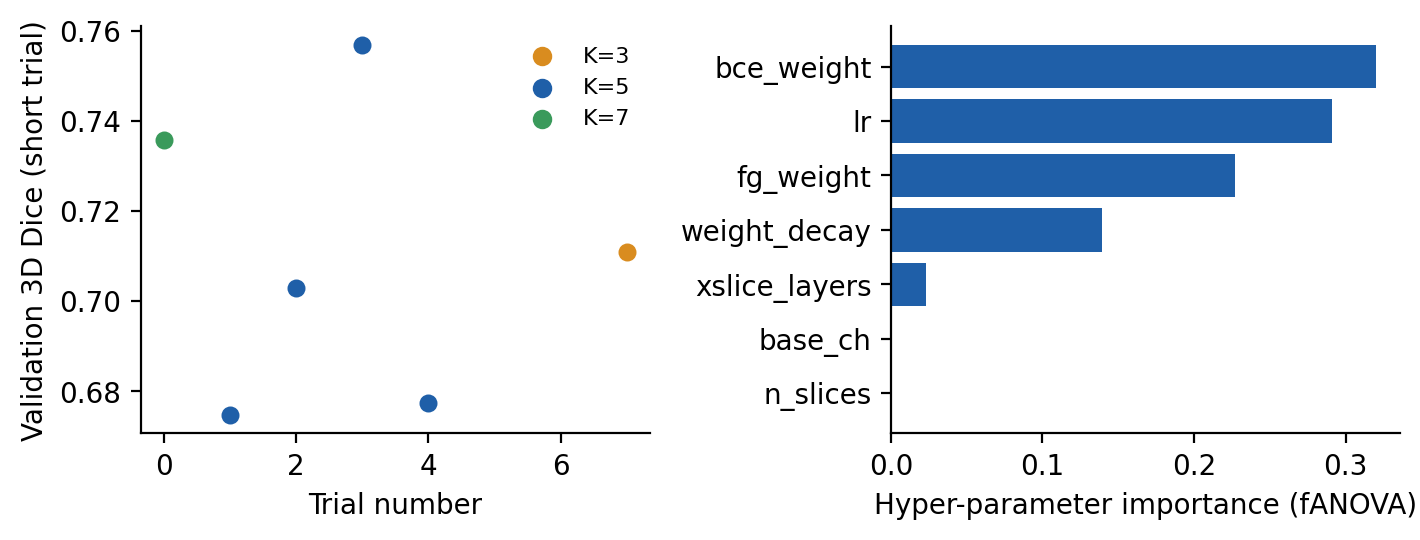
\includegraphics[width=\textwidth]{figures/optuna.png}
\caption{Optuna search: validation Dice of completed trials coloured by slice count $K$ (left) and hyper-parameter importance (right)}\label{fig:optuna}
\end{figure}

\subsection{Supplementary experiment: long training with early stopping}
Before the main experiment we ran a second protocol overnight. It used the best Optuna settings, a 150-epoch cosine schedule, validation every four epochs and early stopping after 40 epochs without improvement. Two of the five $K=5$ runs (folds 0 and 2) failed with GPU out-of-memory errors, because four trainings shared one 40~GB GPU. For the three folds where both models finished, Table~\ref{tab:long} shows that the two models tied: the pooled paired differences over 221 patients were not significant for any Dice region (WT $+0.000$, TC $-0.009$, ET $-0.015$; $p > 0.09$). This comparison was confounded, however. Early stopping halted the $K=5$ runs after their best epochs of 12 and 16 (folds 1 and 3), roughly at epoch 52--56, while the learning rate of the long schedule was still high. The $K=1$ runs had their best epochs at 40--56 and trained until roughly epoch 80--96. The two models therefore received unequal training, and the cross-slice model mostly missed the low-learning-rate phase in which it gained most in the main experiment. Comparing the protocols also shows that the extra training gave the baseline only a small benefit (mean Dice $+0.005$ on average over the five folds relative to the 30-epoch runs), which indicates that 30 annealed epochs are close to convergence. For these reasons the fixed-length protocol, which gives both models an identical budget, is used for the main conclusions, and this experiment is reported for completeness.

\begin{table}[htbp]\centering\small
\caption{Supplementary long-training experiment with early stopping (folds with both runs completed)}\label{tab:long}
\resizebox{\textwidth}{!}{\begin{tabular}{c|ccc|ccc}\toprule
 & \multicolumn{3}{c|}{\textbf{Baseline ($K=1$)}} & \multicolumn{3}{c}{\textbf{Proposed ($K=5$)}}\\
\textbf{Fold} & Mean Dice & Best epoch & Stopped & Mean Dice & Best epoch & Stopped\\\midrule
1 & 0.835 & 56 & early stop & 0.819 & 16 & early stop\\
3 & 0.850 & 48 & early stop & 0.848 & 12 & early stop\\
4 & 0.874 & 40 & early stop & 0.868 & 92 & early stop\\\bottomrule
\end{tabular}}
\end{table}

\section{Comparative Analysis}
\textbf{Against the matched baseline.} The controlled comparison above is the central comparative result. Under identical data, splits, training budget and settings, adding cross-slice attention improves all three Dice scores by a small but statistically reliable margin and reduces boundary error and false-positive slices more substantially, at a cost of 2.37~M additional parameters and roughly 1.6--2 times the training time.

\textbf{Against the mid-review prototype.} With the corrected pipeline the absolute performance of both models improved. The v1 checkpoints, re-evaluated volumetrically on their own validation split, reached a mean Dice of 0.831 (baseline) and 0.826 (cross-slice). The final system reaches 0.839 and 0.844 averaged over all 369 patients in cross-validation. More importantly, the relative result changed: v1's full-data comparison was a tie in Dice, whereas the corrected protocol shows a consistent, significant advantage for cross-slice context.

\textbf{Against published methods.} Table~\ref{tab:sota} places our results beside published BraTS 2020 results for orientation. The numbers are \emph{not} directly comparable. Published results such as TransBTS were obtained on the official BraTS validation set through the challenge server, whereas ours come from internal five-fold cross-validation on the training set, and the MM-MSCA-AF ``overall'' Dice is not broken down by region in its abstract. Our results nevertheless indicate that a lightweight 2.5D model with fewer than 7~M parameters reaches the same range as recent 3D and hybrid methods on the BraTS regions.

\begin{table}[htbp]\centering\small
\caption{Context against published BraTS 2020 results (different evaluation sets; for orientation only)}\label{tab:sota}
\begin{tabular}{p{4.6cm}p{4.4cm}ccc}\toprule
\textbf{Method} & \textbf{Evaluation} & \textbf{WT} & \textbf{TC} & \textbf{ET}\\\midrule
TransBTS (3D CNN + transformer) \cite{wang2021transbts} & Official validation set & 0.901 & 0.817 & 0.787\\
MM-MSCA-AF \cite{aslam2025} & BraTS 2020 (overall Dice 0.859) & -- & -- & --\\
Baseline 2D U-Net (ours) & 5-fold CV, 369 patients & 0.898 & 0.837 & 0.783\\
Cross-slice transformer (ours) & 5-fold CV, 369 patients & 0.904 & 0.840 & 0.789\\\bottomrule
\end{tabular}
\end{table}

\textbf{Against the base paper.} Abdikenov \emph{et al.} reported that adaptive attention added $+0.006$ Dice in CT lymph-node segmentation \cite{abdikenov2026}. Our adaptation to MRI yields a Dice gain of the same order ($+0.005$ mean, $+0.006$ for WT and ET). It also shows clearer improvements in boundary accuracy and slice consistency, which the base paper did not measure in the same way.

\section{Discussion and Interpretation}
The results answer the research question in a nuanced but positive way. Cross-slice attention does make 2.5D glioma segmentation more accurate than an otherwise identical 2D network, and the improvement is consistent across patients and folds. Its size in Dice, however, is modest, about half a Dice point. This is plausible: Dice is dominated by the bulk of large tumours, which a strong 2D network already segments well from a single slice. Neighbouring slices matter most where the evidence in the centre slice is ambiguous, near the top and bottom of the tumour, at thin boundaries and in small enhancing regions. Errors there have little effect on overlap but a large effect on boundary distance and on whether spurious tumour appears on a slice. This is exactly where the cross-slice model gains most: 23\% lower WT boundary error, 15\% lower ET boundary error and a third fewer slices with false-positive tumour.

These findings support the motivation of the project. The objective was not only higher overlap but segmentations that are consistent through the volume, and the HD95 and false-positive-slice results provide direct, statistically tested evidence for that property. For the intended application, consistent boundaries and fewer spurious detections on healthy slices are what reduce a clinician's correction effort, so this kind of improvement matters more in practice than its Dice value suggests. The cost is moderate: the model remains under 7~M parameters and trains in about two hours on one GPU, far below the memory and time demands of the 3D methods in Chapter~3.

The project also produced a methodological lesson. Under the mid-review protocol the comparison appeared to be a tie on full data, and in the supplementary long-training experiment unequal early stopping again produced a tie. Only when the evaluation followed BraTS conventions, the data were normalised per patient, and both models received identical, fully annealed training did a consistent difference emerge. Conclusions about small architectural gains are therefore very sensitive to evaluation and training protocol. This is why we report both experiments and base our claims on paired tests over all patients rather than on a single favourable run.

\section{Limitations}
Several limitations qualify these findings. First, each configuration was trained once per fold with a single seed, so seed-to-seed variance is not quantified, and the Dice improvement (about 0.005) is comparable to typical seed variation in segmentation networks. The paired test over 369 patients establishes consistency across patients for the trained models but not robustness to retraining. Second, performance was estimated by internal cross-validation on the BraTS 2020 training set; results on the official validation set, other BraTS editions or external clinical data were not measured. Third, the Optuna search was short (ten trials, one hour), so its importance estimates are unreliable, and its best setting was not used in the main experiment because that setting was only tested in the confounded long-training protocol. Fourth, the cross-slice module attends over learned bottleneck features. This is a deliberate variant of the base paper's descriptor-based fusion of raw slices, and the paper-faithful variant was not implemented for comparison. Fifth, the gain in TC Dice is small and inconsistent across folds (two of five), and fold 1 shows a small loss in mean Dice. Sixth, no qualitative visual assessment by clinicians, no 3D reference model trained under the same conditions and no measurement of inference time in a clinical workflow were carried out. Finally, the work uses a public research dataset and makes no claim of clinical validity.
